 \chapter{Grundlagen}
Im ersten Teil dieses Kapitels werden die theoretischen Grundlagen, welche in den folgenden Kapitel dieser Arbeit Verwendung finden, erläutert. Als erstes erfolgt eine kurze Einführung in maschinelles Lernen mit Neuronalen Netzen und Deep Learning. Danach wird eine spezielle Form dieser Netzwerke vorgestellt, das sogenannte \emph{Convolutional Neural Network}. Zuletzt wird noch kurz auf das sogenannte \emph{Distant Supervision} \cite{go2009twitter} eingegangen und dieses in Kontext mit der gegebenen Fragestellung (vgl. \ref{introduction}) gesetzt.\\\\
Im zweiten Teil wird auf die Anforderungen sowie die Implementation der Software zum Durchführen der Experimente eingegangen.

\section{Definitionen}

\subsection{Domäne}
Texte, welche die gleiche Struktur aufweisen werden zu einer Domäne zusammengefasst. Als Beispiele lassen sich hier Produktbewertungen, Tweets oder auch Nachrichtentexte erwähnen.\fixme{Stimmt so nicht, nur Volltext und Kurznachricht}

\subsection{Sentiment}
Der \emph{Sentiment} beschreibt das subjektive Empfinden, welches ein Text bei einem Leser auslöst. Im Rahmen dieser Arbeit werden  die drei Sentiments \emph{positiv}, \emph{neutral} und \emph{negativ} verwendet (vgl. Beispiele in Tabelle \ref{basics:sentiments_example_table}). Je nach Bedürfniss lässt sich diese Skala natürlich noch weiter verfeinern, so z.B. mit \emph{eher negativ} oder \emph{eher positiv} als Sentiments.\\
\begin{table}[h]
	\centering
	\begin{tabular}{@{}ll@{}}
		\toprule
		Sentiment & Beispiel\\ \midrule
		positiv & Die Akkulaufzeit dieser Digitalkamera ist aussergewöhnlich hoch.\\
		&\\
		neutral & Dieser Stein ist grau.\\
		&\\
		negativ & Die Auflösung dieser Digitalkamera ist aussergewöhnlich schlecht.\\
		\bottomrule
	\end{tabular}
	\caption{Beispiele für verschiedene Sentiments von Texten}
	\label{basics:sentiments_example_table}
\end{table}
\fixme{Bessere Beispiele!}

Da der Sentiment eines Textes nach dem subjektiven Empfinden einer Person bestimmt wird ist dieser auch nicht eindeutig. Je nachdem wer einen Text beurteilt kann also ein anderes Ergebnis zur Folge haben. Ein Sentiment kann für einzelne Sätze, Abschnitte oder ganze Texte bestimmt werden. Im Rahmen dieser Arbeit ist mit Sentiment immer der Sentiment eines einzelnen Satzes gemeint.

\subsection{Crossdomain}
Mit \emph{Crossdomain} (dt. domänenübergreifend) \fixme{complete!}
\section{Neuronale Netze}
\label{basics:neural_network}
Neuronale Netzwerke sind ein Modell des maschinellen Lernens, welches biologisch motiviert ist und sich lose am menschlichen Gehirn orientiert. Im folgenden wird auf die einzelnen Komponenten eines neuronal Netzwerkes eingegangen.
\subsection{Neuron / Perceptron}
\label{basic:neural_network:neuron}
Die Grundelemente eines neuronalen Netzwerks sind die sogenannten Neuronen, auch Perceptron genannt. Diese Neuronen stellen im Grundsatz nichts anderes als eine mathematische Funktion dar. Der erste wichtige Teil eines Neurons sind die $n + 1$ Eingänge und die mit diesen Eingängen verknüpfte Gewichte ${w_0, w_1, w_2, ..., w_{n+1}}$. Die Anzahl der Eingänge ist $n+1$ und nicht $n$, da jeweils noch ein Bias-Wert dazugerechnet wird. Dieser wird im Normalfall mit $1$ initialisiert. Der zweite wichtige Teil stellt die Aktivierungsfunktion dar. Diese ist dafür zuständig den Ausgabewert eines Neurons zu normalisieren, sprich in eine vordefinierte Spanne an Werten zu bringen. Diese Spanne ist dabei abhängig von der gewählten Aktivierungsfunktion. Als Beispiele von Aktivierungsfunktionen können $tanh$, $relu$ oder auch die $sigmoid$ Funktion aufgelistet werden.\\\\
Der Ausgabewert $y$ eines Neurons lässt sich bei gegebener Aktivierungsfunktion $\gamma$, den Gewichten $w_n$ und den Eingabewerten $x_n$ wie folgt berechnen:

\begin{equation}
y = \gamma(\sum_{i=0}^{n+1} w_i*x_i)
\end{equation}

Das daraus sich ergebende Resultat wird auch die \emph{Aktivierung} des Neurons genannt. Dies ist der Wert, welcher das Neuron an die nächste Schicht weiterreicht (vgl. \ref{basic:neural_network:layer}).

\begin{figure}
	\centering
	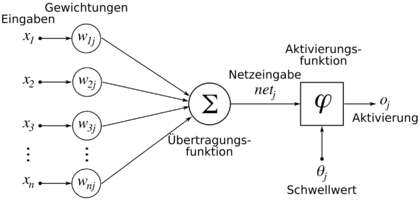
\includegraphics[width=8cm]{img/neuron}
	\caption{Schematische Darstellung eines Neurons}
\end{figure}

\subsection{Schicht}
\label{basic:neural_network:layer}

Um nun ein vollständiges neuronales Netzwerk zu erhalten werden die zuvor erwähnten Neuronen in sogenannten Schichten angeordnet. Dabei gibt es drei essentielle Schichten, welches jedes neuronale Netzwerk hat: Die Eingangsschicht, die Hiddenschicht und die Ausgabeschicht.\\\\

\begin{figure}[h]
	\centering
	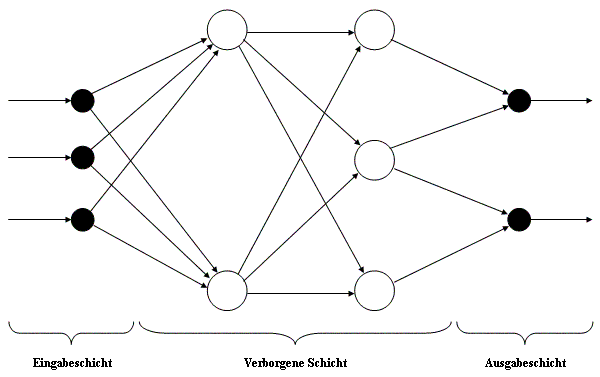
\includegraphics[width=10cm]{img/basic_neural_network}
	\caption{Schematische Darstellung eines neuronalen Netzwerkes}
\end{figure}

Über die Eingabeschicht treten die Eingabedaten $x_1, x_2, ..., x_n$ in das Netzwerk ein. Diese werden dann an die Neuronen der Hiddenschicht vorwärtspropagiert und diese berechnen damit jeweils ihre Aktivierungen. Diese Aktivierungen werden dann von der Hiddenschicht zur Ausgabeschicht weitergereicht wo die sich darin enthaltenen Neuronen wiederum ihre Aktivierung berechnen. Die Eingabewerte der einzelnen Neuronen der Ausgabeschicht sind dabei die Aktivierungen aller Neuronen der vorhergehenden Schicht. Dieser Vorgang des "Vorwärtsrechnens" wird auch als Vorwärtspropagierung bezeichnet. Bei einem neuronalen Netzwerk mit mehr als einer Hiddenschicht spricht man auch von einem \emph{Deep Neural Network}.\\\\
Die Anzahl der Neuronen und ihre Aktivierungen in der Ausgabeschicht hängt von der konkreten Problemstellung ab. Im Falle dieser Arbeit sind in der Ausgabeschicht drei Neuronen vorhanden, wobei jedes für einen bestimmten Sentiment steht.

\subsection{Backpropagation}
Wie bei fast allen Modelle des maschinellen Lernens, lernt das neuronale Netztwerk mittels dem optimieren einer Fehlerfunktion. Das Optimieren dieser Fehlerfunktion wird mittels dem \emph{Backpropagation}-Algorithmus erzielt. Als Fehlerfunktion kann jede Funktion dienen, mit welcher der Aussagefehler des Netzwerks quanitifiziert werden kann. Als Beispiele können hier der MSE, MAE oder auch Categorical Cross-Entropy aufgeführt werden. Der Algorithmus kann in den folgenden Schritten zusammegefasst werden:
\begin{enumerate}
	\item Die Eingabedaten in das Netzwerk einführen und die Vorwärtspropagierung durch-führen.
	\item Die Ausgabedaten des Netzwerks werden mit dem erwarteten Resultat verglichen. Die Differenz des Ausgabewertes vom erwarteten Wert wird als Fehler des Netzwerkes bezeichnet.
	\item Der Fehler wird nun durch das neuronale Netzwerk hindurch zurückpropagiert. Dabei werden die Gewichte der einzelnen Schichten abhängig von ihrem Einfluss auf den berechneten Fehler verändert.
\end{enumerate}

Die Berechnung des Einfluss eines einzelnen Gewichtes auf den Fehler wird mittels der partiellen Ableitung der Fehlerfunktion bezüglich dem entsprechenden Gewicht festgestellt. Danach wird das Gewicht neu berechnet indem man den Wert der partiellen Ableitung mal der Lernrate vom aktuellen Gewicht subtrahiert. Das neue Gewicht für das Neuron $i$ in der Schicht $k$ berechnet sich bei gegebener Lernrate $\eta$ und Fehlerfunktion $E$ also wie folgt:

\begin{equation}
w_{ik} = w_{ik} - \eta \frac{\delta E}{\delta w_{ik}}
\end{equation}

Alle partiellen Ableitungen nach allen Gewichten der Fehlerfunktion wird auch Gradient genannt. Dies wird nun für jedes Neuron der Hidden- und Ausgabeschicht berechnet und die Gewichte werden entsprechend angepasst. Die Lernrate $\eta$ beschreibt dabei, wie gross der Einfluss eines einzelnen Backpropagation-Durchlaufs auf die Gewichte des neuronalen Netzwerks hat. Dabei wird der errechnete Gradient mit der Lernrate multipliziert. Entsprechend führt eine Lernrate $\eta > 1.0$ dazu dass der Gradient vergrössert bzw. mit $\eta < 1.0$ verkleinert wird.
\subsubsection{AdaDelta}
Backpropagation besitzt das Problem, dass der Erfolg des Algorithmus stark von der gewählten Lernrate $\eta$ abhängt. Bei einer zu grossen Lernrate wird das Optimum möglicherweise übersprungen oder der Werte der Fehlerfunktion divergiert sogar, bei einer zu kleinen Lernrate dauert es sehr lange bis das Optimum der Fehlerfunktion gefunden wird.\\

\begin{figure}[h]
	\centering
	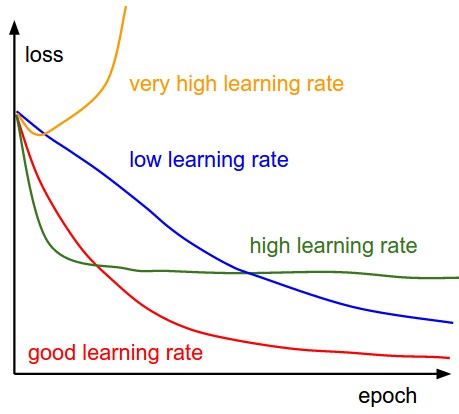
\includegraphics[width=6cm]{img/learning_rates_comparison}
	\caption{Beispielhafte gegenüberstellung verschiedener Lernraten\protect\footnote{http://cs231n.github.io/assets/nn3/learningrates.jpeg}}
\end{figure}

\emph{AdaDelta} \cite{zeiler2012adadelta} ist eine verfeinerte Version der Grundform des Backpropagation-Algorithmus und eine weiterentwicklung von \emph{AdaGrad}. Der grosse Vorteil von AdaDelta ist, dass keine Lernrate definiert werden muss. \fixme{More infomrations!}
\section{Convolutional Neural Network}
\emph{Convolutional Neural Networks}, abgekürzt \gls{cnn}, sind eine spezielle Form der in \ref{basics:neural_network} beschriebenen neuronalen Netzen. Der Unterschiede der beiden Arten liegt darin, dass bei einem CNN die einzelnen Schichten nicht vollkommen miteinander verbunden sind (nicht \emph{fully-connected}), sondern mittels Filter über lokale Konnektivität versucht wird Muster zu erkennen.
\subsection{Filter}
\label{basic:cnn:filter}
Anstatt Neuronen wie im klassischen Neuronalen Netzwerk (vgl. \ref{neural_network:basics:neuron}) lernt eine CNN über die sogenannten Filter. Dabei handelt es sich um $n\times m$-Matrizen, welche Gewichte enthalten, analog zu den Gewichten der eingehenden Verbindungen bei Neuronen. Dabei werden die Filter-Matrizen über die Eingabedaten bewegt und es wird jeweils das innere Produkt der aktuellen Filter-Matrix und dem aktuellen Ausschnitt der Eingabedaten berechnet auf welchem der Filter positioniert ist. Das Bewegungsmuster des Filters wird \emph{Stride} (dt. durchschreiten) genannt. Im Rahmen dieser Arbeit wird nur ein eindimensionaler Stride entlang der Satz-Matrix (vgl. \ref{missing!}) verwendet.\\\\
Die durch diese Convolutions resultierende Werte werden der Form einer Resultat-Matrix, der sogenannten \emph{Feature Map}, zwischengespeichert. Diese stellen also das Äquivalent zur Aktivierung einer Schicht im klassischen Neuronalen Netzwerk (vgl. \ref{basic:neural_network:layer}) dar. Dabei werden alle resultierenden Feature-Maps einfach hintereinandergereiht und dienen als Eingabewerte für die nächste Schicht. 

\begin{figure}[h]
	\centering
	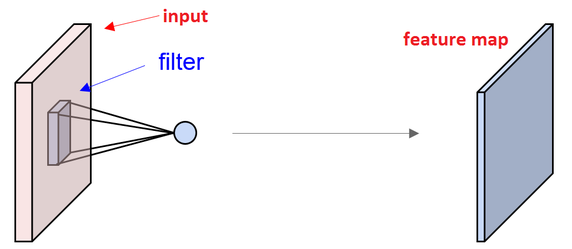
\includegraphics[width=10cm]{img/filter_feature_map}
	\caption{Schematische Darstellung Filter und Feature-Map}
\end{figure}

Diese wird in der Pooling-Schicht (vgl. \ref{basic:cnn:pooling}) weiterverarbeitet. Eine Schicht, welche diese Art von Berechnung verwendet wird auch Convolutional (dt. Fallten) Schicht genannt.
\subsection{Zero-Padding}
\blindtext

\subsection{Max-Pooling Schicht}
\label{basic:cnn:pooling}
In der \emph{Max-Pooling} Schicht wird ein grossteil der in den Feature-Maps vorhandenen Informationen verworfen. Dabei wird ein Fenster über die resultierenden Feature-Maps der vorhergehenden Schicht bewegt und der jeweils maximale Wert des entsprechenden Ausschnitts der aktuellen Feature-Map als Wert in die gepoolte Represäntation übernommen. Das Fenster, welches über die Feature-Map bewegt wird, ist definiert durch die Dimensionalität des Fensters und dem Stride. Dieser steht für das Bewegunsmuster des Fenster analog zum Filter (vgl. \ref{basic:cnn:filter}). Die gepoolte Represäntationen der Feature-Maps dienen dann als Eingabewerte für die nächste Convolutional Schicht.\\\\

\begin{figure}[h]
	\centering
	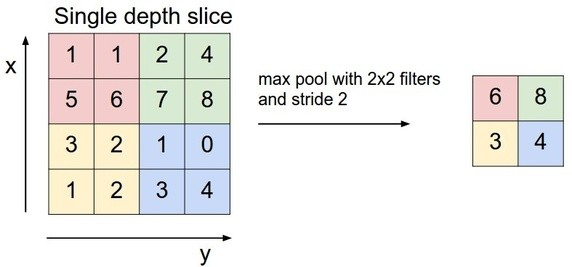
\includegraphics[width=10cm]{img/max_pooling}
	\caption{Schematische Darstellung der Max-Pooling Schicht}
\end{figure}

Der Vorgang in der Max-Pooling Schicht wird auch als \emph{sub-sampling} bezeichnet.

\subsection{Convolutional+Max-Pooling Schicht}
Die Convolutional und Max-Pooling Schicht bilden die Grundbausteine eines CNN. Diese werden nun mehrfach hintereinander gereiht. Das im Rahmen dieser Arbeit vewendete CNN hat als Beispiel zwei solcher aufeinanderfolgenden Convolutional+Max-Pooling Schichten.\\

\begin{figure}[h]
	\centering
	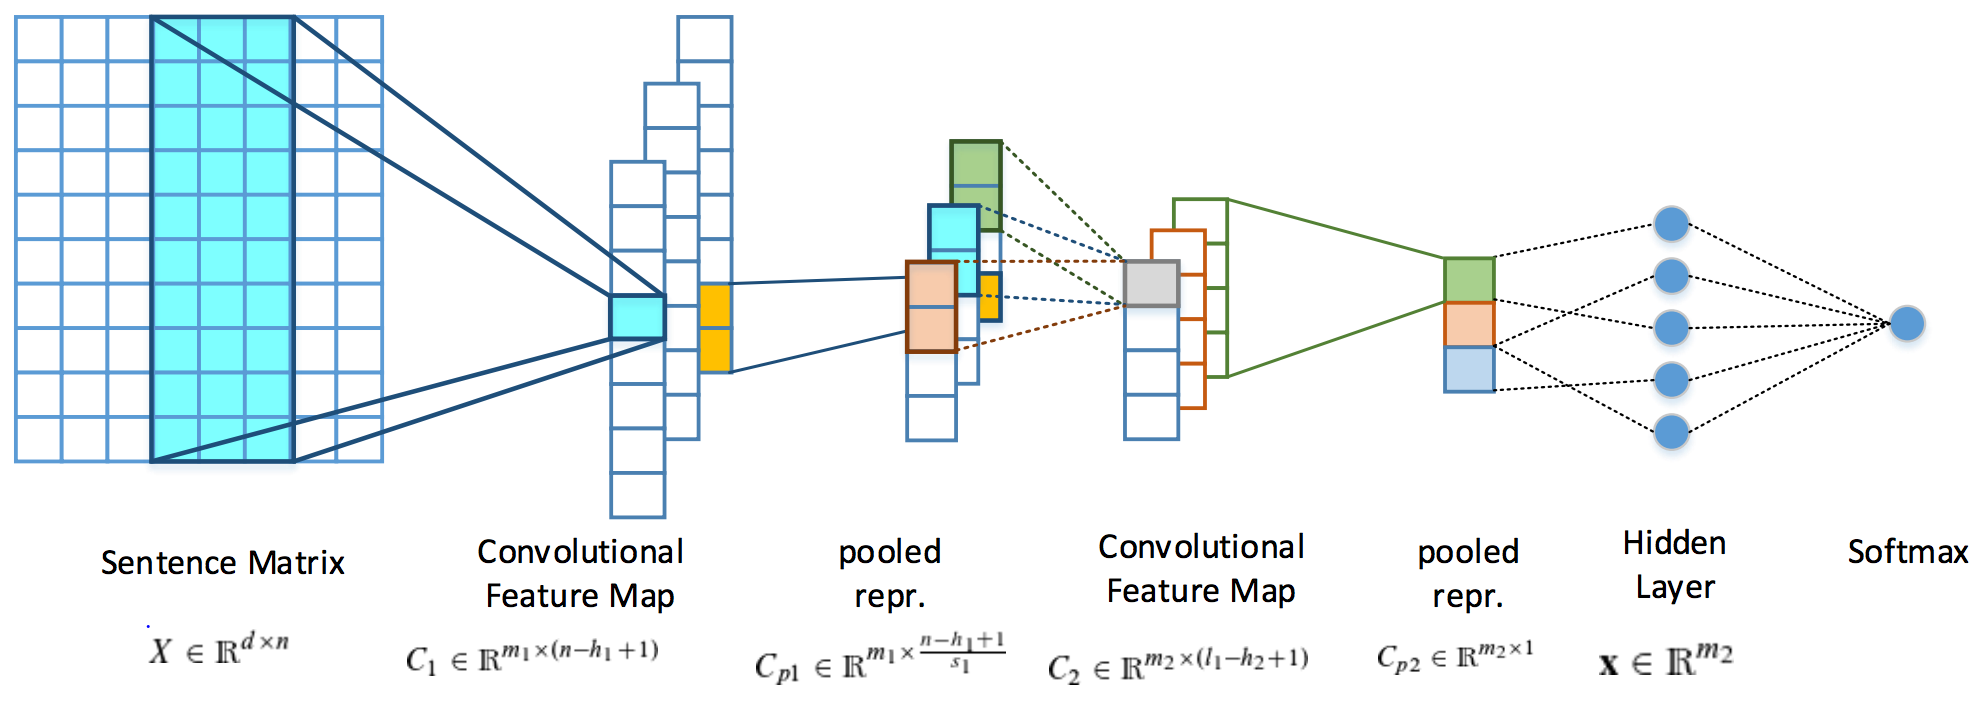
\includegraphics[width=10cm]{img/semeval_cnn_structure}
	\caption{Schematische Darstellung des in dieser Arbeit verwendeten CNN \protect\cite{deriu2016swisscheese}}
\end{figure}

\subsection{Ausgabeschicht}
Am Ende des CNN wird eine fully-connected Schicht angehängt. Diese funktioniert genau gleich wie bereits beim Neuronalen Netzwerk beschrieben wurde (vgl. \ref{basic:neural_network:layer}). Dabei stehen die einzelnen Neuronen der Ausgabeschicht für die einzelnen Klassen, welche detektiert werden sollen. Im Falle des in dieser Arbeit verwendeten CNN gibt es in der Ausgabeschicht drei Neuronen wobei jeder für einen der entsprechenden Sentiments steht..
\section{Word Embeddings}

\section{Distant Supervision}
Wie bereits in \ref{basics:neural_network} erläutert benötigen NNs, vor allem CNNs, sehr viele annotierte Trainingsdaten \fixme{Referenz} um am Ende des Trainings ein zufriedenstellendes Modell zu erhalten. Ein grossteil der vorhandenen Datensätze umfassen allerdings nicht mehr als 10'000 Texte. Des Weiteren sind die Sentiments in diesen Datensätzen sehr oft nicht gleichverteilt. Das führt dazu, dass gewisse Sentiments unterrepräsentiert sind, während andere überdurchschnittlich oft vorhanden sind. Im Falle der in dieser Arbeit verwendeten Datensätze ist es so, dass der positive und negative Sentiment unterdurchschnittlich oft vorkommen, während es überdurchschnittlich viele Texte mit einem neutralen Sentiment gibt (vgl. \ref{data:supervised_data}). Dadurch lernt das CNN zwar sehr gut Texte mit neutralem Sentiment zu erkennen, allerdings tut es sich sehr schwer mit den anderen beiden Sentiments.
\fixme{mehr informationen!}
\section{Metriken}
Um einen Klassifizierer zu bewerten werden die folgend beschriebenen Metriken verwendet.
\subsection{Präzision {\&} Ausbeute}
\label{basics:metrics:precision_recall}

\subsection{F1-Score}
Die in \ref{basics:metrics:precision_recall} beschriebenen Metriken Präzision und Ausbeute haben ein fundamentales Problem: Wenn die Klassen ungleich verteilt sind kann eine hohe Präzision bzw. Ausbeute erreicht werden indem einfach immer die am stärksten vertretene als Resultat zurückgegeben wird.\\\\Am Beispiel der Testdaten aus den JCR{\_}quotations (vgl. \ref{data:supervised_data}) ist einfach ersichtlich wo das Problem liegt. Der neutrale Sentiment ist hier überdurchschnittlich hoch vertreten mit $66.9\%$. Wenn der Klassifizierer also immer also Resultat den neutralen Sentiment zurückgibt führt das automatisch zu einer Ausbeute von $100\%$ und einer Präzision von $66.9\%$. Dies entspricht zwar der Realität ist aber irreführend.\\\\
Um dieses Problem zu umgehen wird im Rahmen dieser Arbeit der F1-Score verwendet. Diese wird als Kombination der Präzision und der Ausbeute mithilfe der Gleichung \ref{basic:metrics:f1_eq} berechnet.

\begin{equation}
\label{basic:metrics:f1_eq}
F1 = \frac{2*precision*recall}{precision + recall}
\end{equation}

Der zusammengefasste F1-Score über die zwei Klassen $x$ und $y$ wird mithilfe der Gleichung \ref{basic:metrics:f1_comb_eq} berechnet.

\begin{equation}
\label{basic:metrics:f1_comb_eq}
F1_{x|y} = \frac{F1_x + F1_y}{2}
\end{equation}

\section{Technische Implementation}
Im folgenden Abschnitt wird der technische Aufbau, welcher verwendet wurde, um die in \ref{experiments} beschriebenen Experimente durchzuführen.

\subsubsection{Vorarbeiten}
\label{technichal_setup:prework}
Der Grundaufbau der verwendeten Software wurde von Jan Deriu mithilfe von Keras\footnote{https://keras.io/} implementiert und zur Durchführung dieser Arbeit zur Verfügung gestellt. Im Rahmen dieses Grundaufbaus wurde die folgende Funktionalität bereits implementiert:

\begin{itemize}[noitemsep]
	\item Implementation des CNN in Keras und verwendung von Theano \cite{theanoCitShort} als Backend für die GPUs (vgl. Abschnitt \ref{technichal_setup:hardware}).
	\item Implementation von Evaluations-Metriken
	\item Skripte mit den folgenden Funktionalitäten: Trainieren des CNN, Laden von TSV Dateien, Vorverarbeiten von Word-Embeddings
\end{itemize}

\subsubsection{Anforderungen}
\label{technical_setup:requirements}
Ein System, welches die in \ref{experiments} beschriebenen Experimente durchführen kann, soll die folgenden Eigenschaften aufweisen:

\begin{itemize}
	\item \textbf{Parametrisierbarkeit}: Dadurch dass eine grosse Anzahl kleiner Experimente durchgeführt werden muss soll das System die Möglichkeit bitten Experimente parametrisiert durchzuführen.
	\item \textbf{Wiederholbarkeit}: Experimente sollen wenn nötig mehrfach durchgeführt werden ohne einen Mehraufwand zu verursachen. 
	\item \textbf{Übersichtlichkeit}: Resultate der Experimente sollen übersichtlich und einfach zugänglich sein.
	\item \textbf{Auswertbarkeit}: Resultate sollen \fixme{Bessers Wort für Einfach?} einfach ausgewertet werden können.
\end{itemize}

Die in \ref{technichal_setup:prework} beschriebenen Vorarbeiten bitten eine Basis um damit ein System aufzubauen, welches die oben beschriebenen Eigenschaften aufweist.
\subsubsection{Funktionalität}
\label{technical_setup:functionality}
Um ein System, welches die im vorhergehenden Kapitel beschriebenen Eigenschaften aufweist, zu erhalten, wurden die folgenden Komponenten implementiert:

\begin{itemize}
	\item \textbf{Executor}: Der \emph{Executor} ist zuständig für das Training der CNNs mithilfe von Keras. Beim Start akzeptiert er die Konfiguration als Parameter. Das Experiment wird mit dem Laden der benötigten Daten und dem anschliessenden Trainings des CNN gestartet. Am Ende jeder Epoche wird das aktuelle CNN auf den Validierungsdaten getestet und die konfigurierten Metriken ausgewertet. Diese werden am Ende zusammen mit dem trainierten CNN (Gewichte im HDF5-Format\footnote{https://support.hdfgroup.org/HDF5/}, das CNN Model als JSON) in einen für das Experiment vorgesehenen Ordner gespeichert. Die Metriken werden ebenfalls in diesem dem dafür vorgesehenen Ordner abgespeichert.
	\item \textbf{Config Management}: Experimente werden über Konfigurationen im JSON-Format\footnote{http://www.json.org/} parametrisiert. Über diese Konfiguration können viele wichtige Parameter für die Ausführung festgelegt werden, so zum Beispiel: Anzahl Epochen, Trainings- und Validierungsdaten, Parameter für k-fold Cross-Validation oder auch bereits Trainierte Modelle können geladen werden. Für eine vollständige Liste wird auf den Quellcode des Projektes verwiesen. Experimente können mittels der group{\_}id gruppiert werden. Damit können die Experimente hierarchisch mittels zwei Ebenen gruppiert werden.
	\item \textbf{DataLoader}: Mithilfe des \emph{DataLoader} können Trainings- und Validierungsdaten im TSV\footnote{https://reference.wolfram.com/language/ref/format/TSV.html} Dateiformat geladen werden. Die zu ladenden Daten können dabei aus einer oder mehreren TSV-Dateien stammen. Im Falle das mehrere TSV Dateien angegeben werden kann über die Konfiguration das Verhältnis angegeben werden, in welchem die Daten aus den einzelnen Dateien verschmischt werden sollen.
	\item \textbf{Skripte}: Die Auswertung der einzelnen Experimente geschieht über dafür erstelle Skripte (vgl. \ref{technical_setup:scripts}).
	\item \textbf{Weboberfläche}: Auf die Resultate der Experimente können über eine eigens dafür entwickelte Weboberfläche zugegriffen werden. Ausserdem besteht die Möglichkeit Plots über die Metriken welche während des Trainings- und Validierungsprozess gesammelt wurden auszuwerten (vgl. \ref{technical_setup:webgui}).
\end{itemize}
\fixme{Referenze auf Code, Code-Style bei group{\_}id}
Die oben beschriebenen Komponenten erlauben es Experimente mittels JSON Konfigurationen zu starten und den gesamten Trainings- und Validierungsprozess mittels der Metriken zu dokumentieren.

\subsubsection{Skripte}
\label{technical_setup:scripts}
Für die Durchführung der Experimente wurden diverse Skripte erstellt um die Handhabung zu vereinfachen und Auswertungen zu ermöglichen. Die Liste der implementierten Script umfasst unter anderem die folgenden:

\begin{itemize}[noitemsep]
	\item Erstellen von Plots der Lernkurven und Metriken
	\item Erstellen von Word-Embeddings über einen Textcorpus
	\item Erstellen von Statistiken zu Trainings- und Validierungsdaten
	\item Vorverarbeitung von Trainingsdaten für die Distant-Phase
	\item Erstellen von Visualisierungen von Word-Embeddings mittels t-SNE \cite{maaten2008visualizing}.
	\item Diverse Wartungsscripkte zur Generierung und Verwaltung von Experimenten
\end{itemize}

\subsubsection{Weboberfläche}
\label{technical_setup:webgui}
Um die dritte Anforderung nach Übersichtlichkeit und Auswertbarkeit (vgl. \ref{technical_setup:requirements}) zu erfüllen wurde eine Weboberfläche umgesetzt, mit welchem die Parameter und Resultate aller durchgeführten Experimente übersichtlich und an einem Ort zur Verfügung gestellt werden. Für die Implementation wurde das Python Framework flask\footnote{http://flask.pocoo.org/} verwendet.\fixme{Bilder der Weboberfläche, Schrift flask}\\
Zur Auswertung der Experimente stehen drei Funktionen zur Verfügung:
\begin{itemize}
	\item Die Oberfläche gewährt Zugriff auf alle JSON Konfigurationen, welche zu einem Experiment gehören. Dazu zählen die Konfiguration selbst, die gespeicherten Trainings- und Validierungsmetriken und das CNN Model (vgl. \ref{technical_setup:functionality}).
	\item Mittels der Plotting Funktion können Plots von Trainingsmetriken erstellt werden. Weiterhin können Plots und Boxplots über die die Validierungsmetriken der einzelnen Schritte der Crossdomain-Experimente (vgl. \ref{methods:v8}) erstellt werden.
	\item Die gespeicherten Validierungs- und Trainingsmetriken können mithilfe von math.js\footnote{http://mathjs.org/} direkt im Browser ausgewertet werden.\fixme{Code-Style}
\end{itemize}
\begin{figure}[htbp]
	\centering
	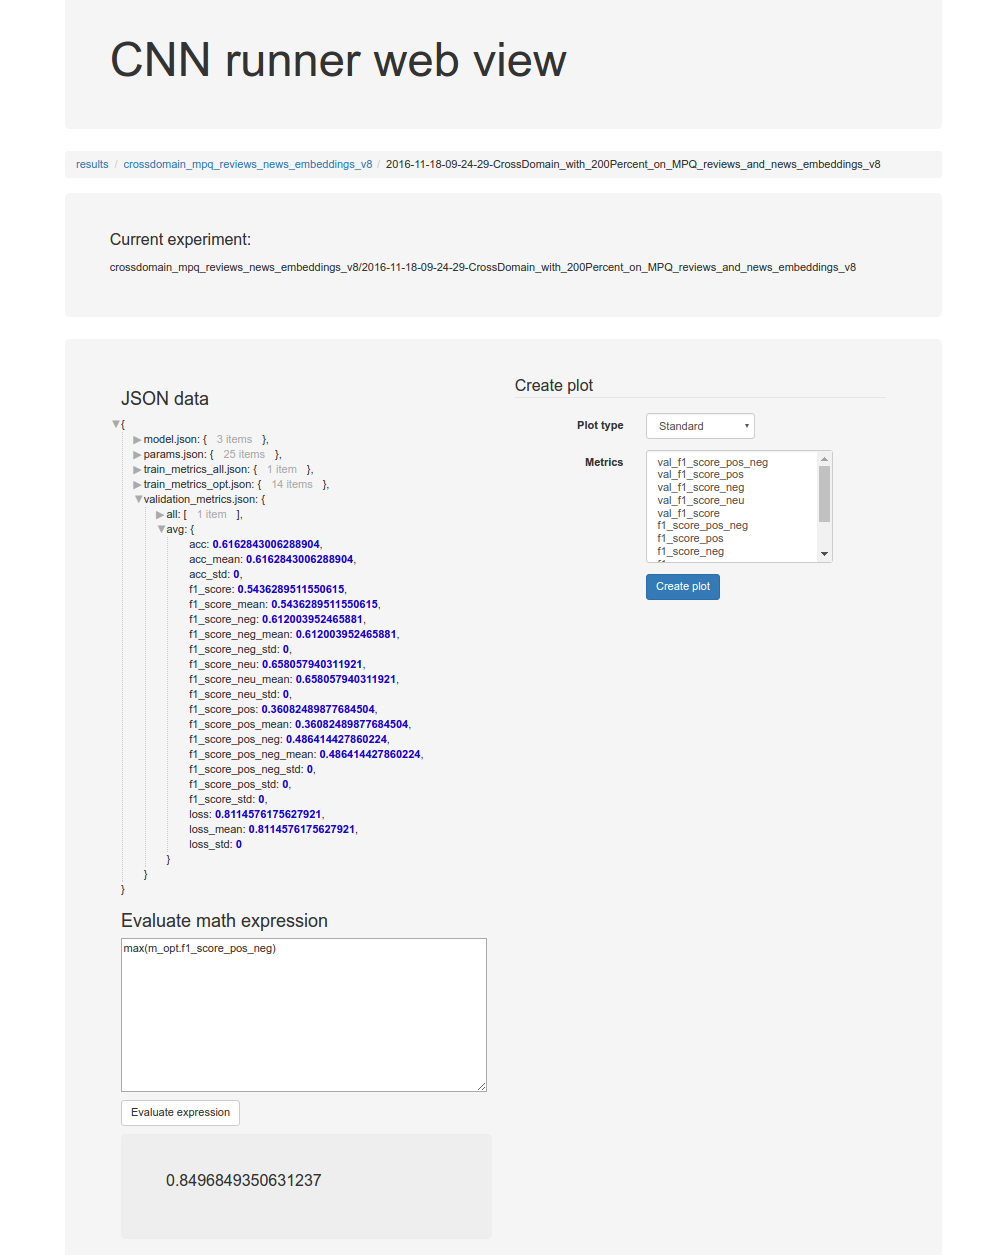
\includegraphics[width=0.7\textwidth]{img/web_gui}
	\caption{Ansicht Experiment über Weboberfläche}
	\label{fig:web_gui}
\end{figure}
\subsubsection{Betriebssystem \& Softwarepakete}
\label{technical_setup:software}
Alle Experimente wurden mit der unten beschriebenen Implementation durchgeführt. Auf beiden verwendeten Computer-Systemen (vgl. \ref{technichal_setup:prework}) wurde als Betriebssystem Ubuntu 16.04 installiert. Dazu wurden Python 3.5.2\footnote{https://www.python.org/}, Nvidia GPU Treiber und cuda8\footnote{https://developer.nvidia.com/cuda-toolkit} als Abhängigkeiten von Theano und Keras installiert.

\subsection{Hardware}
\label{technichal_setup:hardware}
Zur Durchführung der Experimente wurden zwei unterschiedliche Computer verwendet. Im ersten System (S1) ist eine Nvidia GTX970 GPU, einen Intel i7 4950K CPU und 16GB Arbeitsspeicher installiert. Das zweite System besitzt eine Nvidia GTX1070 GPU, einen Intel i7 6700K CPU und ebenfalls 16GB Arbeitsspeicher. Die Unterschiede in der Hardware haben keinen Einfluss auf die Experimente, da auf beiden System dasselbe Betriebssystem mit den gleichen Softwarepaketen verwendet wurde (vgl. \ref{technical_setup:software}).

